% Options for packages loaded elsewhere
\PassOptionsToPackage{unicode}{hyperref}
\PassOptionsToPackage{hyphens}{url}
%
\documentclass[
]{article}
\usepackage{amsmath,amssymb}
\usepackage{lmodern}
\usepackage{iftex}
\ifPDFTeX
  \usepackage[T1]{fontenc}
  \usepackage[utf8]{inputenc}
  \usepackage{textcomp} % provide euro and other symbols
\else % if luatex or xetex
  \usepackage{unicode-math}
  \defaultfontfeatures{Scale=MatchLowercase}
  \defaultfontfeatures[\rmfamily]{Ligatures=TeX,Scale=1}
\fi
% Use upquote if available, for straight quotes in verbatim environments
\IfFileExists{upquote.sty}{\usepackage{upquote}}{}
\IfFileExists{microtype.sty}{% use microtype if available
  \usepackage[]{microtype}
  \UseMicrotypeSet[protrusion]{basicmath} % disable protrusion for tt fonts
}{}
\makeatletter
\@ifundefined{KOMAClassName}{% if non-KOMA class
  \IfFileExists{parskip.sty}{%
    \usepackage{parskip}
  }{% else
    \setlength{\parindent}{0pt}
    \setlength{\parskip}{6pt plus 2pt minus 1pt}}
}{% if KOMA class
  \KOMAoptions{parskip=half}}
\makeatother
\usepackage{xcolor}
\usepackage[margin=1in]{geometry}
\usepackage{graphicx}
\makeatletter
\def\maxwidth{\ifdim\Gin@nat@width>\linewidth\linewidth\else\Gin@nat@width\fi}
\def\maxheight{\ifdim\Gin@nat@height>\textheight\textheight\else\Gin@nat@height\fi}
\makeatother
% Scale images if necessary, so that they will not overflow the page
% margins by default, and it is still possible to overwrite the defaults
% using explicit options in \includegraphics[width, height, ...]{}
\setkeys{Gin}{width=\maxwidth,height=\maxheight,keepaspectratio}
% Set default figure placement to htbp
\makeatletter
\def\fps@figure{htbp}
\makeatother
\setlength{\emergencystretch}{3em} % prevent overfull lines
\providecommand{\tightlist}{%
  \setlength{\itemsep}{0pt}\setlength{\parskip}{0pt}}
\setcounter{secnumdepth}{-\maxdimen} % remove section numbering
\ifLuaTeX
  \usepackage{selnolig}  % disable illegal ligatures
\fi
\IfFileExists{bookmark.sty}{\usepackage{bookmark}}{\usepackage{hyperref}}
\IfFileExists{xurl.sty}{\usepackage{xurl}}{} % add URL line breaks if available
\urlstyle{same} % disable monospaced font for URLs
\hypersetup{
  pdftitle={Honolulu accessibility: a preliminary report},
  pdfauthor={JT Keller and Alicia Seeley},
  hidelinks,
  pdfcreator={LaTeX via pandoc}}

\title{Honolulu accessibility: a preliminary report}
\author{JT Keller and Alicia Seeley}
\date{2023-02-21}

\begin{document}
\maketitle

\hypertarget{introduction}{%
\section{Introduction}\label{introduction}}

This report seeks to define and measure accessibility for Honolulu
county.

\hypertarget{definition-of-accessibility-and-explanation-of-specific-accessibility-metric}{%
\subsection{Definition of Accessibility and Explanation of Specific
Accessibility
Metric}\label{definition-of-accessibility-and-explanation-of-specific-accessibility-metric}}

We based our definition of level of accessibility on Susan Handy's
``Enough with the ``D's'' Already --- Let's Get Back to ``A'''' which
asserts that ``the level of accessibility from a given place reflects
the distribution of destinations around it, the ease with which those
destinations can be reached by various modes, and the amount and
character of activity found there.'' For the purpose of this exercise,
the `distribution of destinations' refers to employment locations
relative to a given origin, the `ease with which destinations can be
reached by various modes' is measured through travel times and other
impedance weights (explained below) for driving and bus modes, and
`character of activity' refers specifically to employment.

\hypertarget{metrics}{%
\section{Metrics}\label{metrics}}

\hypertarget{calculating-perceived-travel-time}{%
\subsection{Calculating Perceived Travel
Time}\label{calculating-perceived-travel-time}}

The assumption that most public transit riders are more bothered by
out-of-vehicle waiting time than in-vehicle travel time seems to hold
true for Honolulu. In fact, a bit of searching internet blogs and review
sites (see Figures 1 and 2) revealed that a common complaint about the
bus system was buses running very late or not arriving at all. This adds
additional frustration to long headways. We thus decided to set the
weight for out-of-vehicle time to be 3 times that of in-vehicle time.

\begin{figure}

{\centering 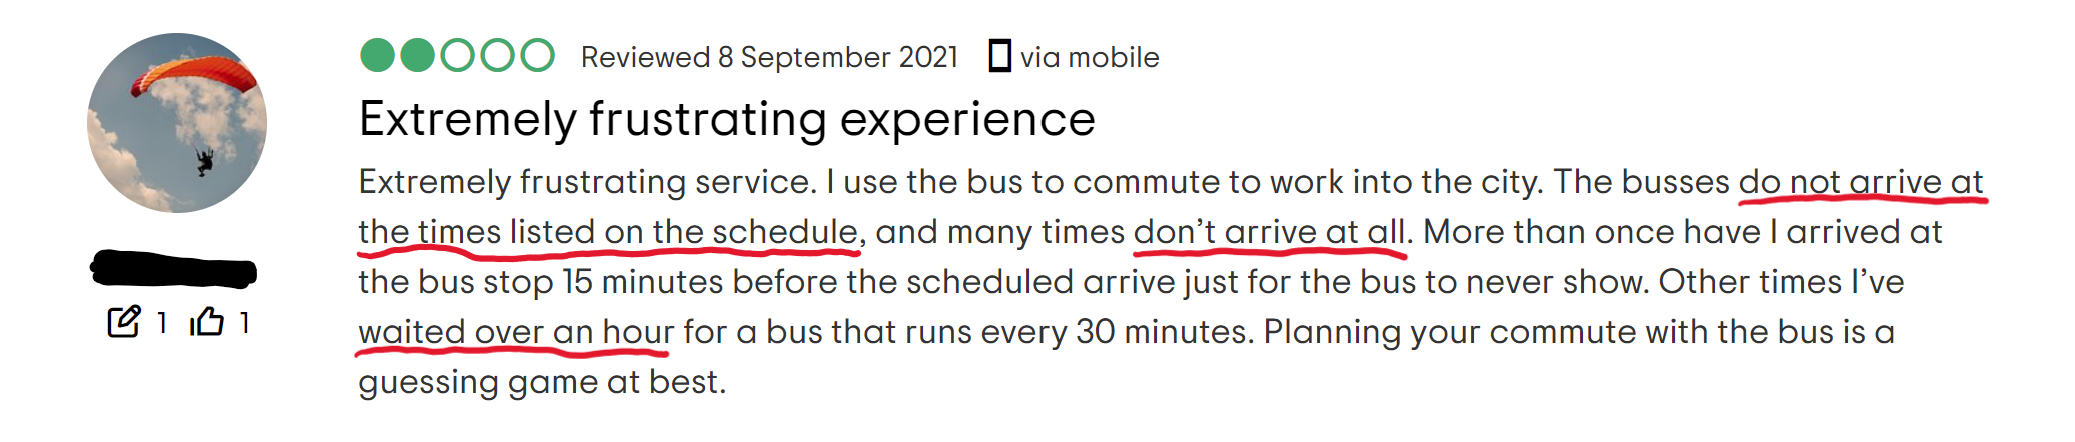
\includegraphics[width=1\linewidth]{A5 Images/Review-1} 

}

\caption{Figure 1: Annotated snapshot of TheBus review from anonymous user, TripAdvisor.com}\label{fig:figurename1}
\end{figure}

\begin{figure}

{\centering 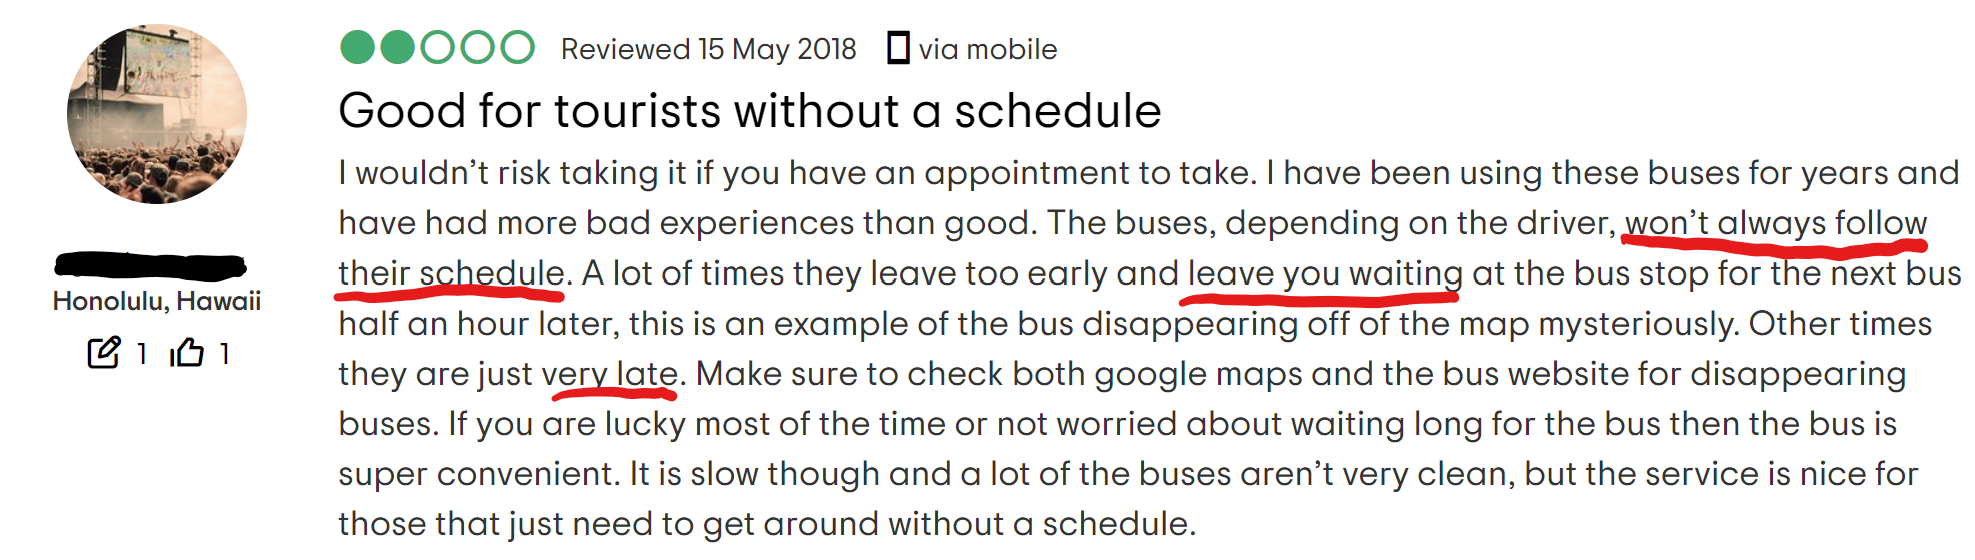
\includegraphics[width=1\linewidth]{A5 Images/Review-2} 

}

\caption{Figure 2: Annotated snapshot of another TheBus review from anonymous user, TripAdvisor.com}\label{fig:figurename2}
\end{figure}

\hypertarget{defining-decay-function}{%
\subsection{Defining Decay Function}\label{defining-decay-function}}

For Honolulu, we chose to use a logistic function to represent decay.
Because of the large variation in travel times and generally long travel
times on buses in Honolulu, we believe that the difference in
accessibility for a 10-minute transit trip versus a 20-minute transit
trip would influence perceived accessibility and impedance more than the
difference between a 90-minute trip and a 100-minute trip, for example
(Since they are already taking such a long bus ride, what is ten more
minutes?), ruling out the logic behind exponential, step, or linear
functions of decay.

We defined an inflection point of 45. Given the wide variability in bus
trip durations across the island and its inconsistency, we believe that
the perceived accessibility is likely to decline at a higher inflection
point than (have a shallower rate of decline) than more urbanized areas
like Boston.

As for standard deviation, we decided on a unit of 10 to account for
variability in users, their respective reasons for traveling, and other
individual characteristics. We thought it best to be generous here
because of the high volume of tourists and visitors who generally have
different standards than residents and daily commuters. This also
relates to the variability in expectations based on geography, as the
urban core is a small part of the island and those traveling within the
urban core will have different perceptions of accessibility compared to
those who start or end their trips in more mountainous or outlying
areas.

\hypertarget{weight-jobs-for-each-origin-destination-pair}{%
\subsection{Weight Jobs For Each Origin-Destination
Pair}\label{weight-jobs-for-each-origin-destination-pair}}

As we start taking car trips into account, we (unsurprisingly) noticed a
wider range in travel times by car. Because of this, we decided to
continue using the logistic decay function, but to adjust the parameters
to have an inflection point of 30 minutes and a standard deviation of 20
because we can assume that drivers are less amenable to longer travel
times. In other words, given their relative independence compared to bus
users, they would most likely expect a more fixed travel time and so the
inflection point would be lower.

\hypertarget{combine-absolute-transit-and-car-access}{%
\subsection{Combine Absolute Transit and Car
Access}\label{combine-absolute-transit-and-car-access}}

We opted not to combine car accessibility with transit accessibility,
keeping them as separate indices. We did not think calculating an
absolute value for overall accessibility would be meaningful in the
context of Honolulu. The island offers only one option for public
transportation, which uses the same road network as cars. Given the
perceived unreliability of the bus, we assume that those with access to
cars will almost always drive because it will always be the more
efficient option. Given these assumptions, we posit that each user would
primarily only use one form of transportation or the other rather than a
mix of the two, and thus an overall accessibility measure would not be
useful.

\hypertarget{results}{%
\section{Results}\label{results}}

\begin{figure}

{\centering 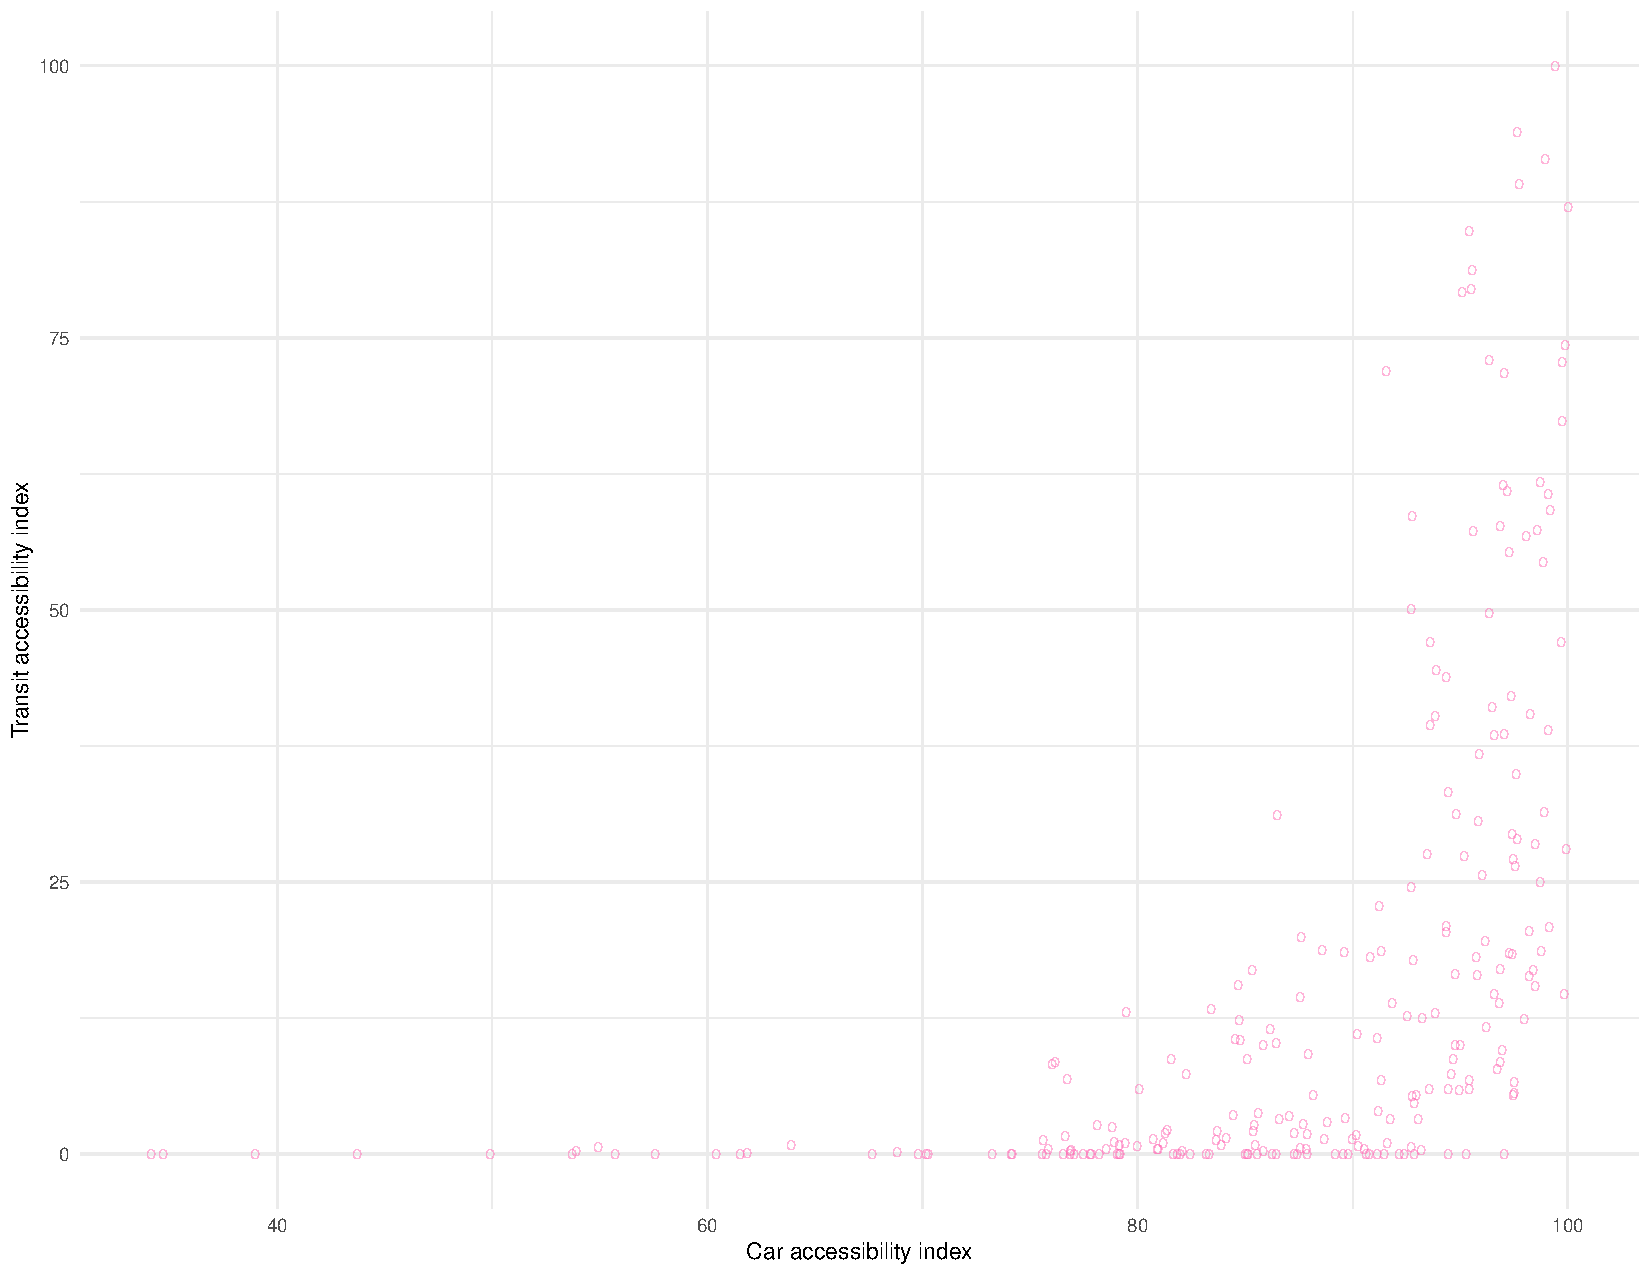
\includegraphics[width=1\linewidth]{access_scatterplot} 

}

\caption{Figure 3: This scatterplot visualizes the heavy skew toward car accessibility relative to transit accessibility. You see a large cluster of points with high car accessibility and zero transit accessibility.}\label{fig:figurename3}
\end{figure}
\begin{figure}

{\centering 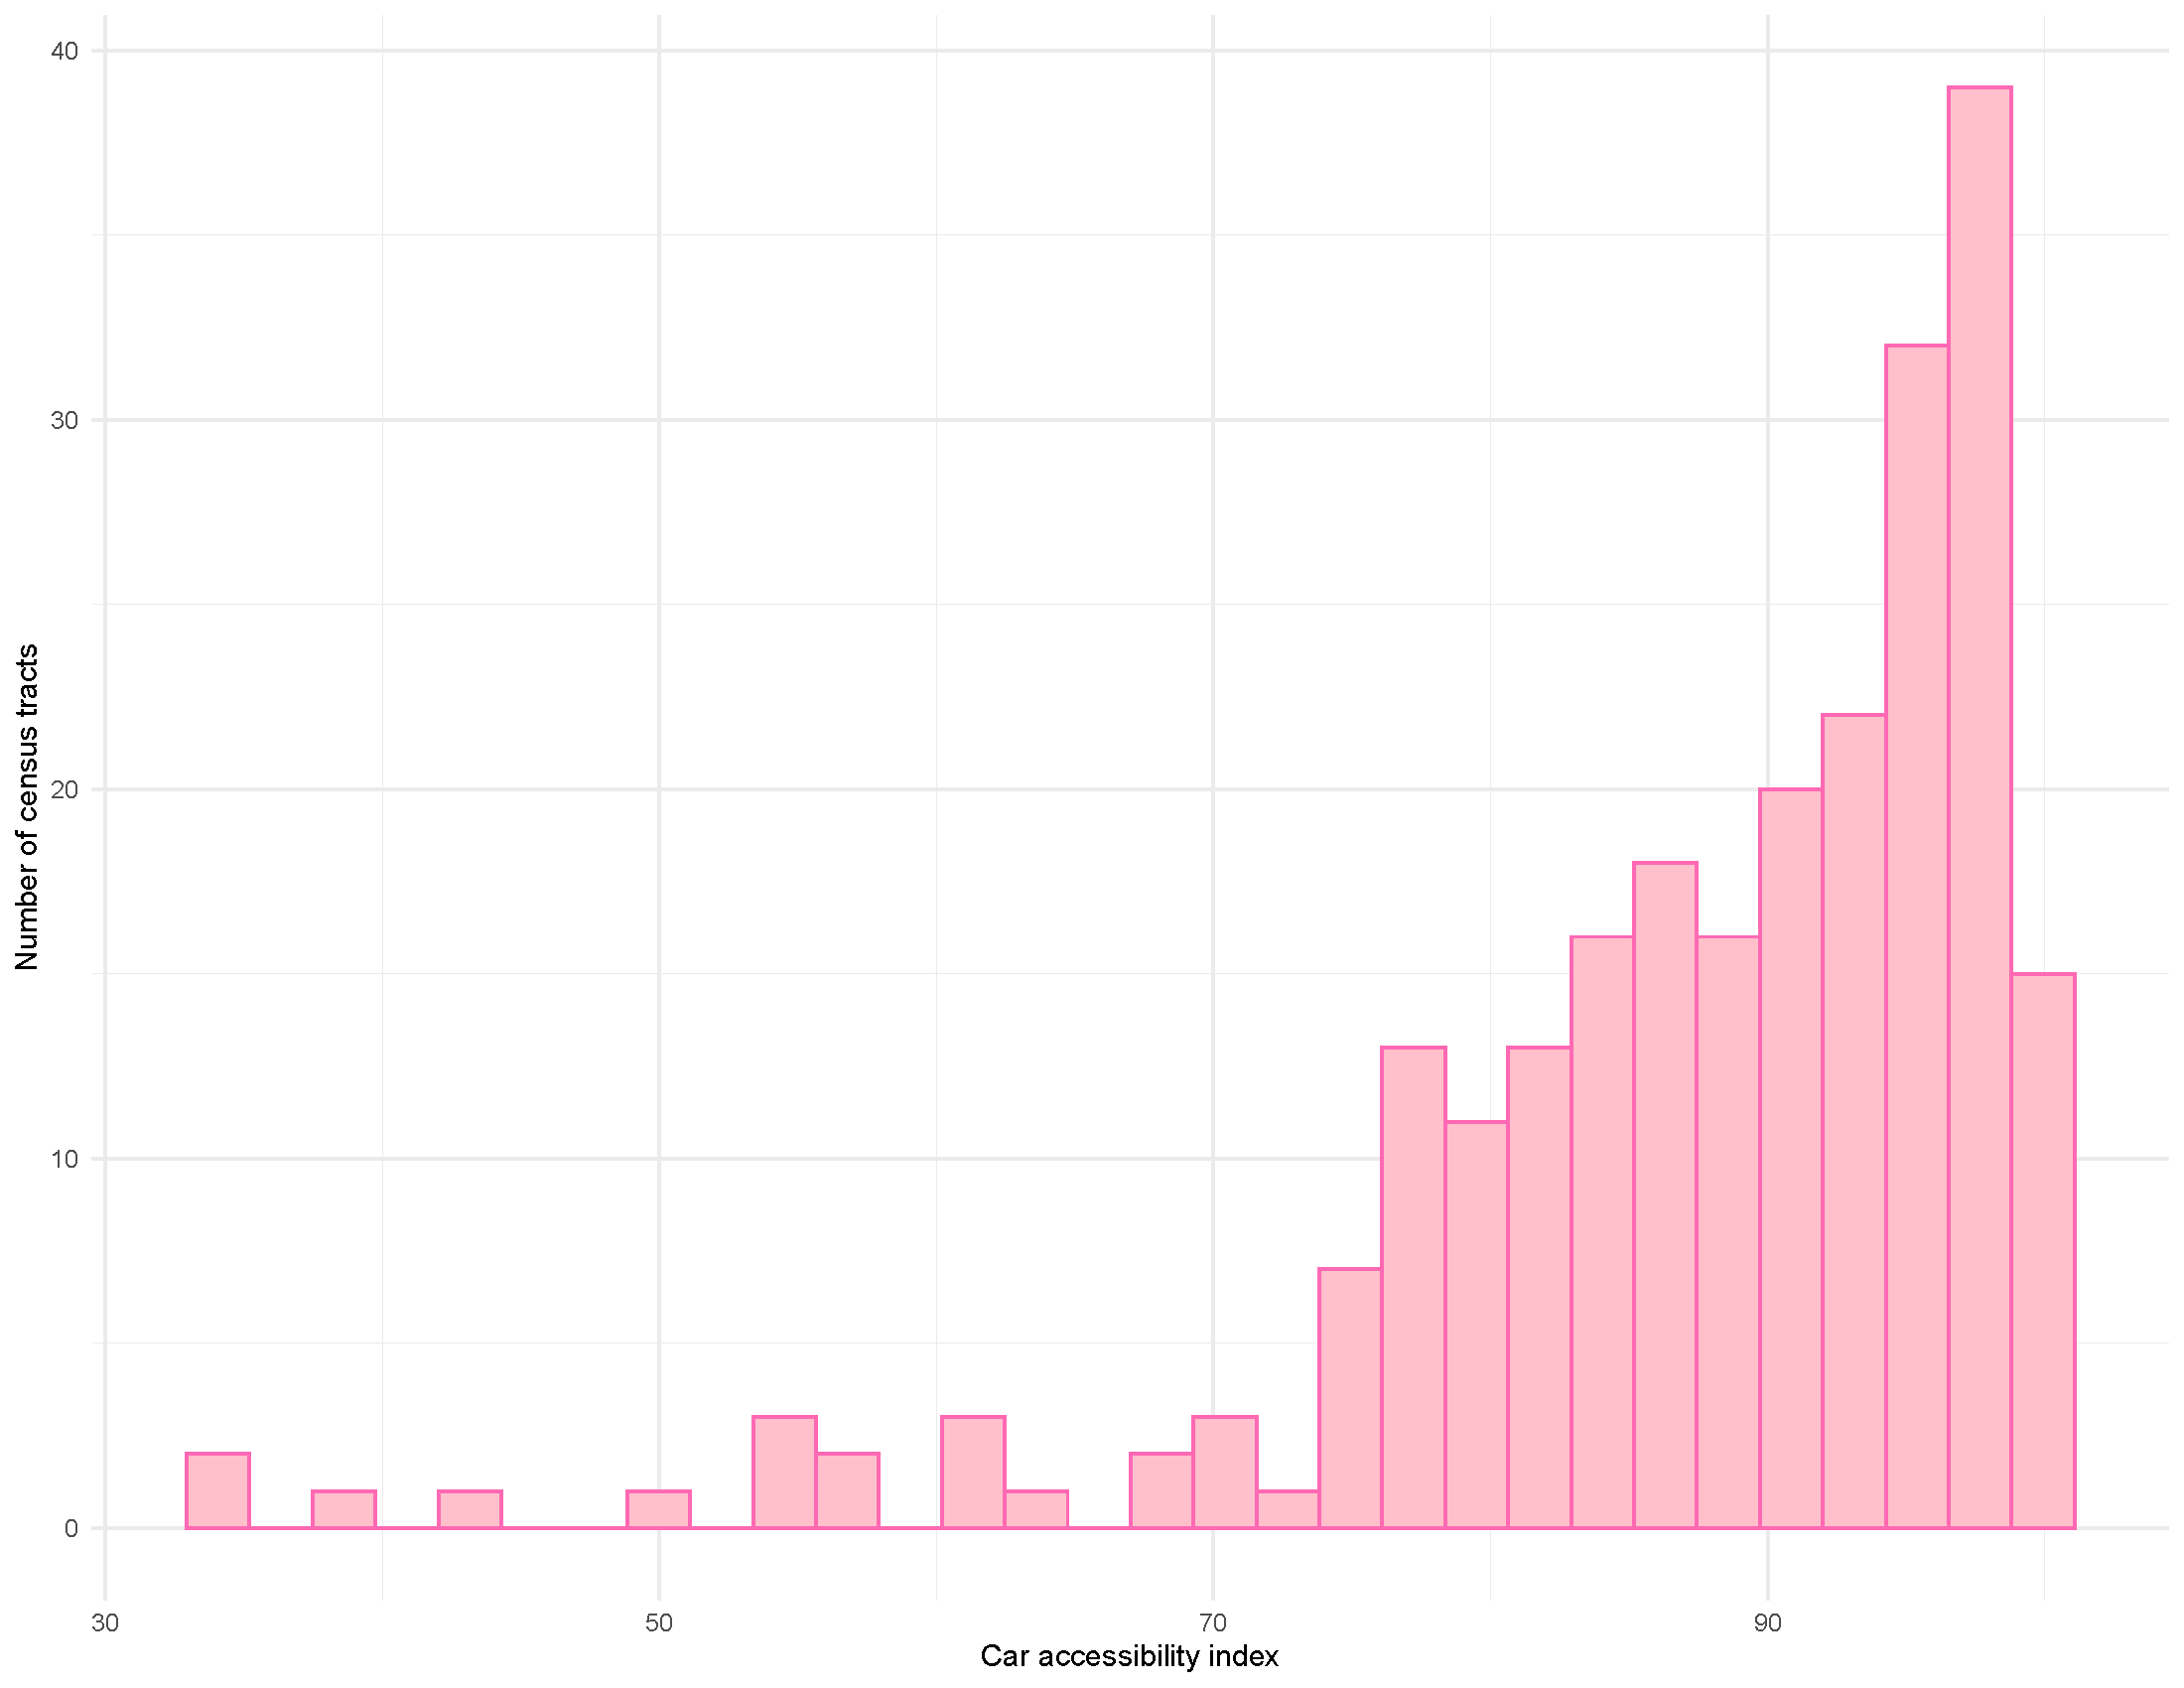
\includegraphics[width=1\linewidth]{car_barchart} 

}

\caption{Figure 4: Car accessibility skews very high}\label{fig:figurename4}
\end{figure}

\begin{figure}

{\centering 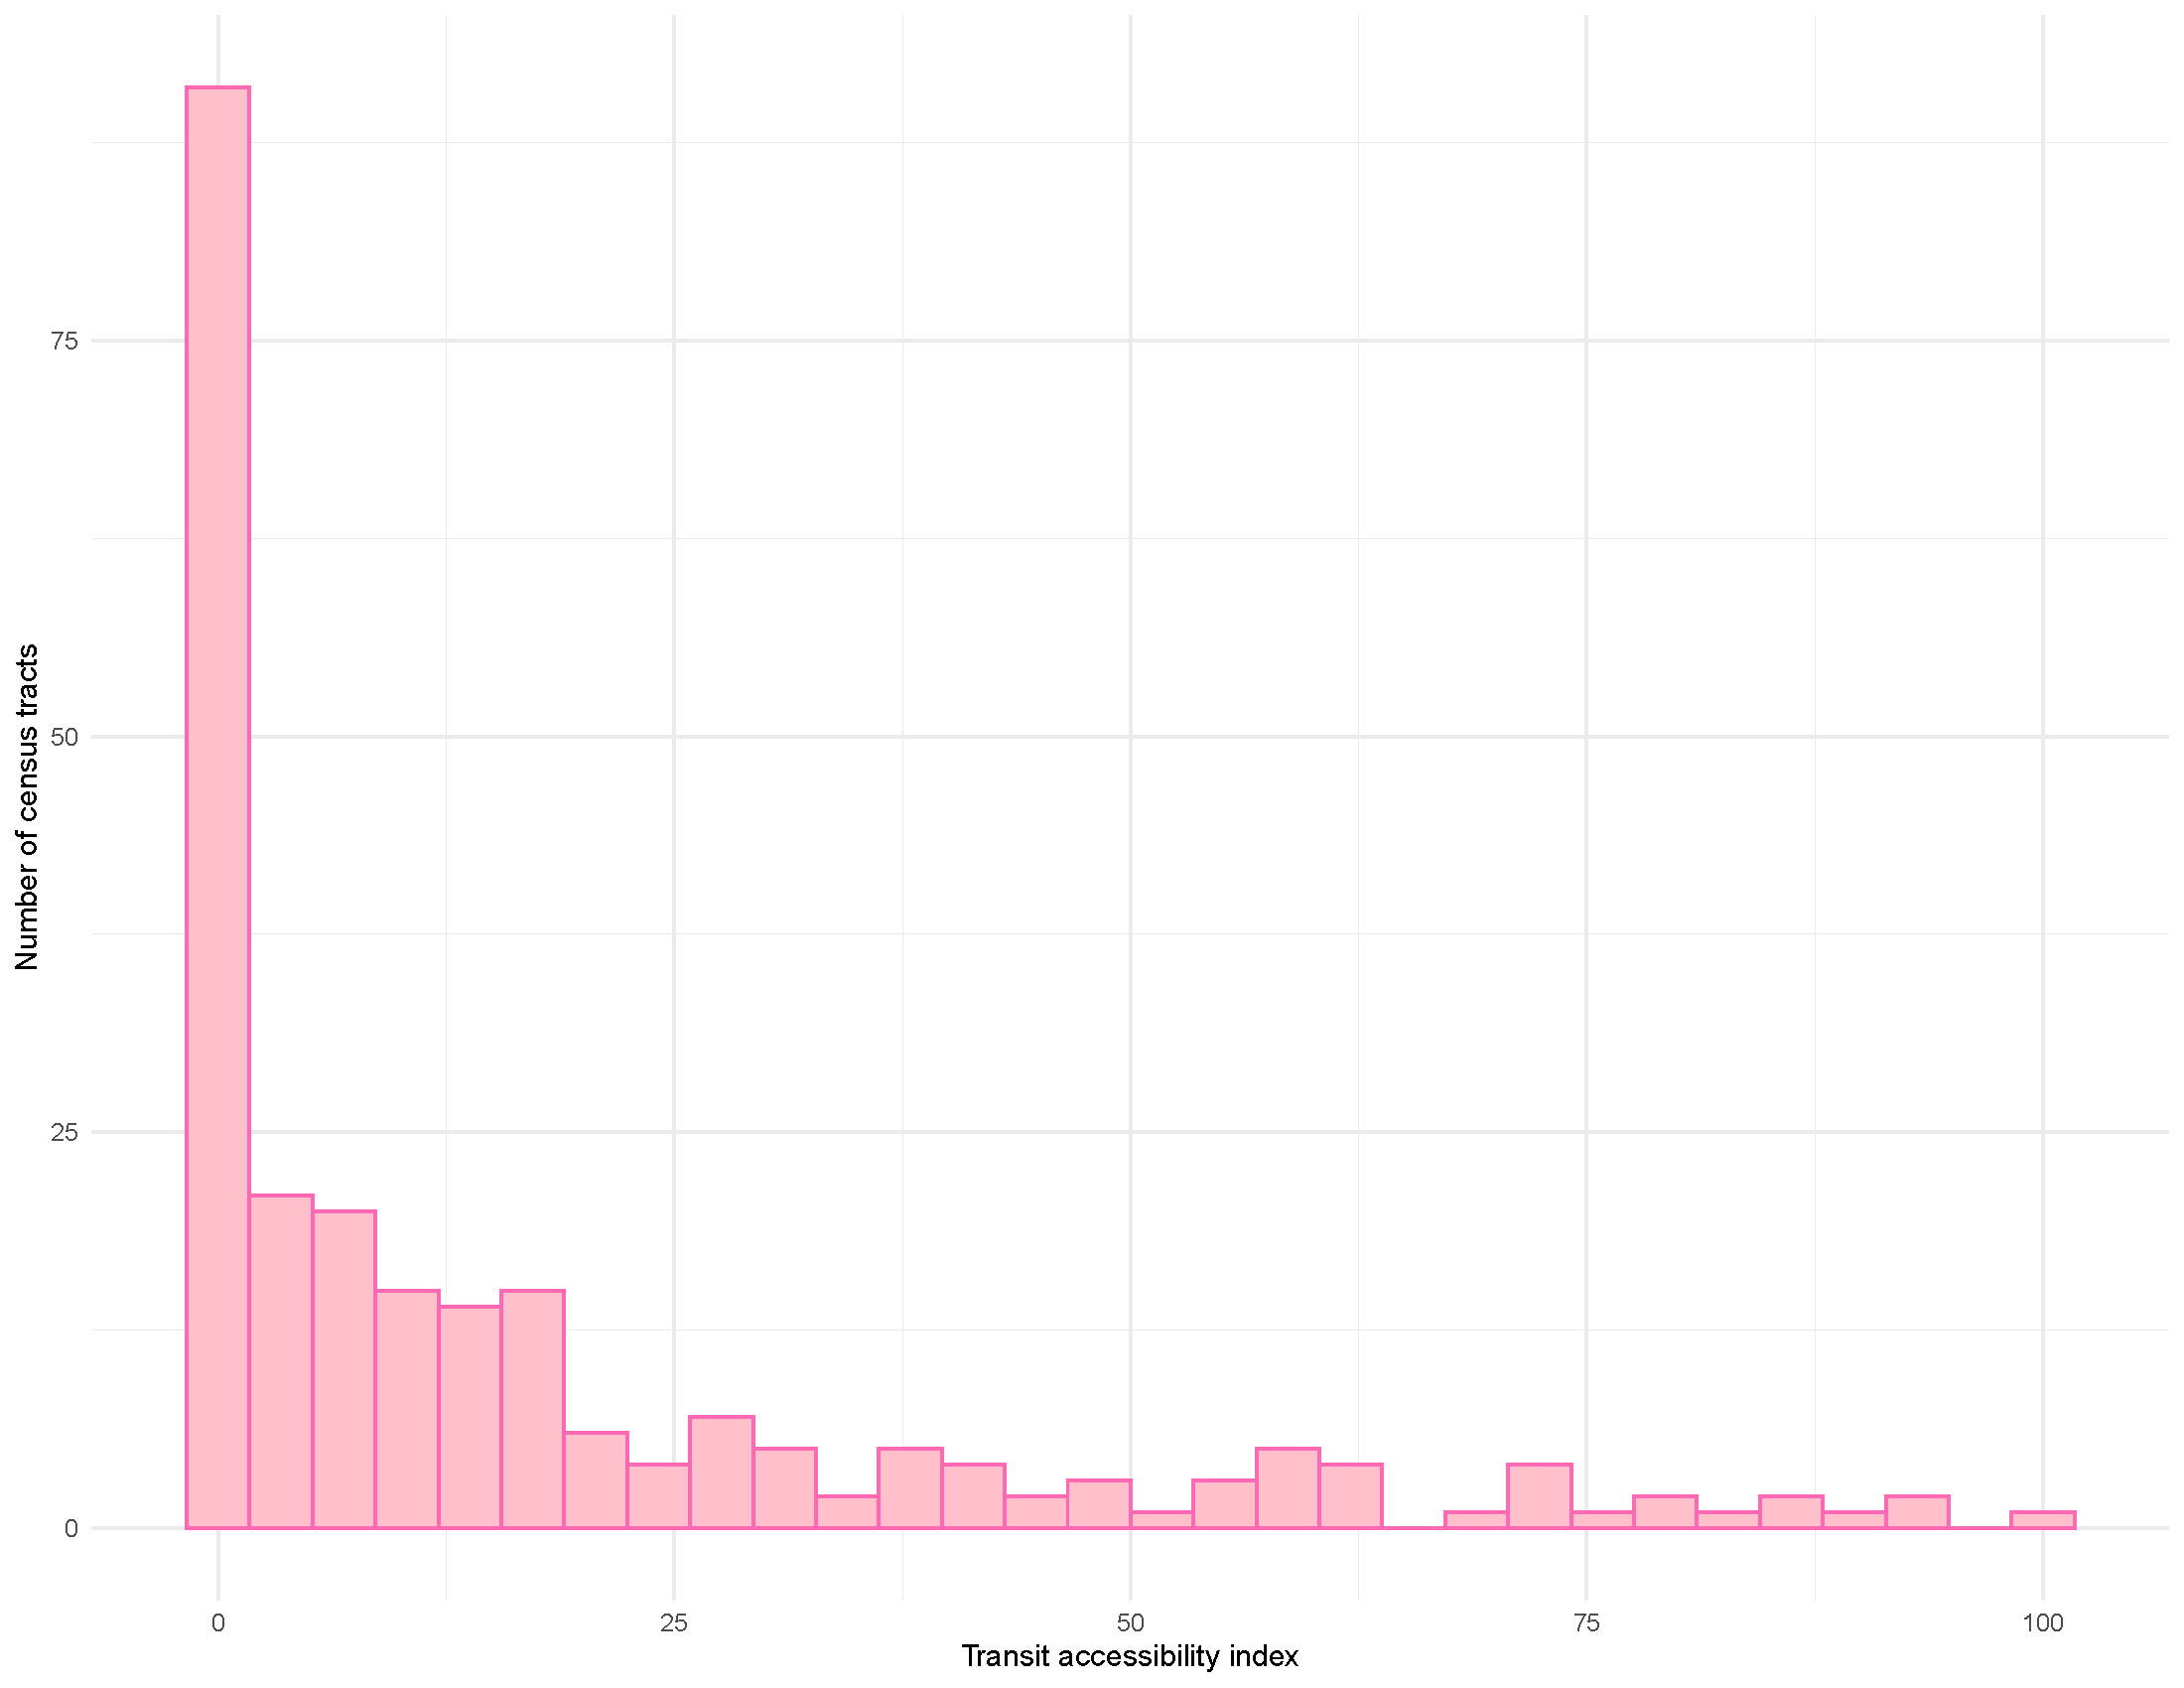
\includegraphics[width=1\linewidth]{transit_barchart} 

}

\caption{Figure 5: Transit accessibility skews very low}\label{fig:figurename5}
\end{figure}

\hypertarget{conclusion}{%
\section{Conclusion}\label{conclusion}}

\begin{figure}

{\centering 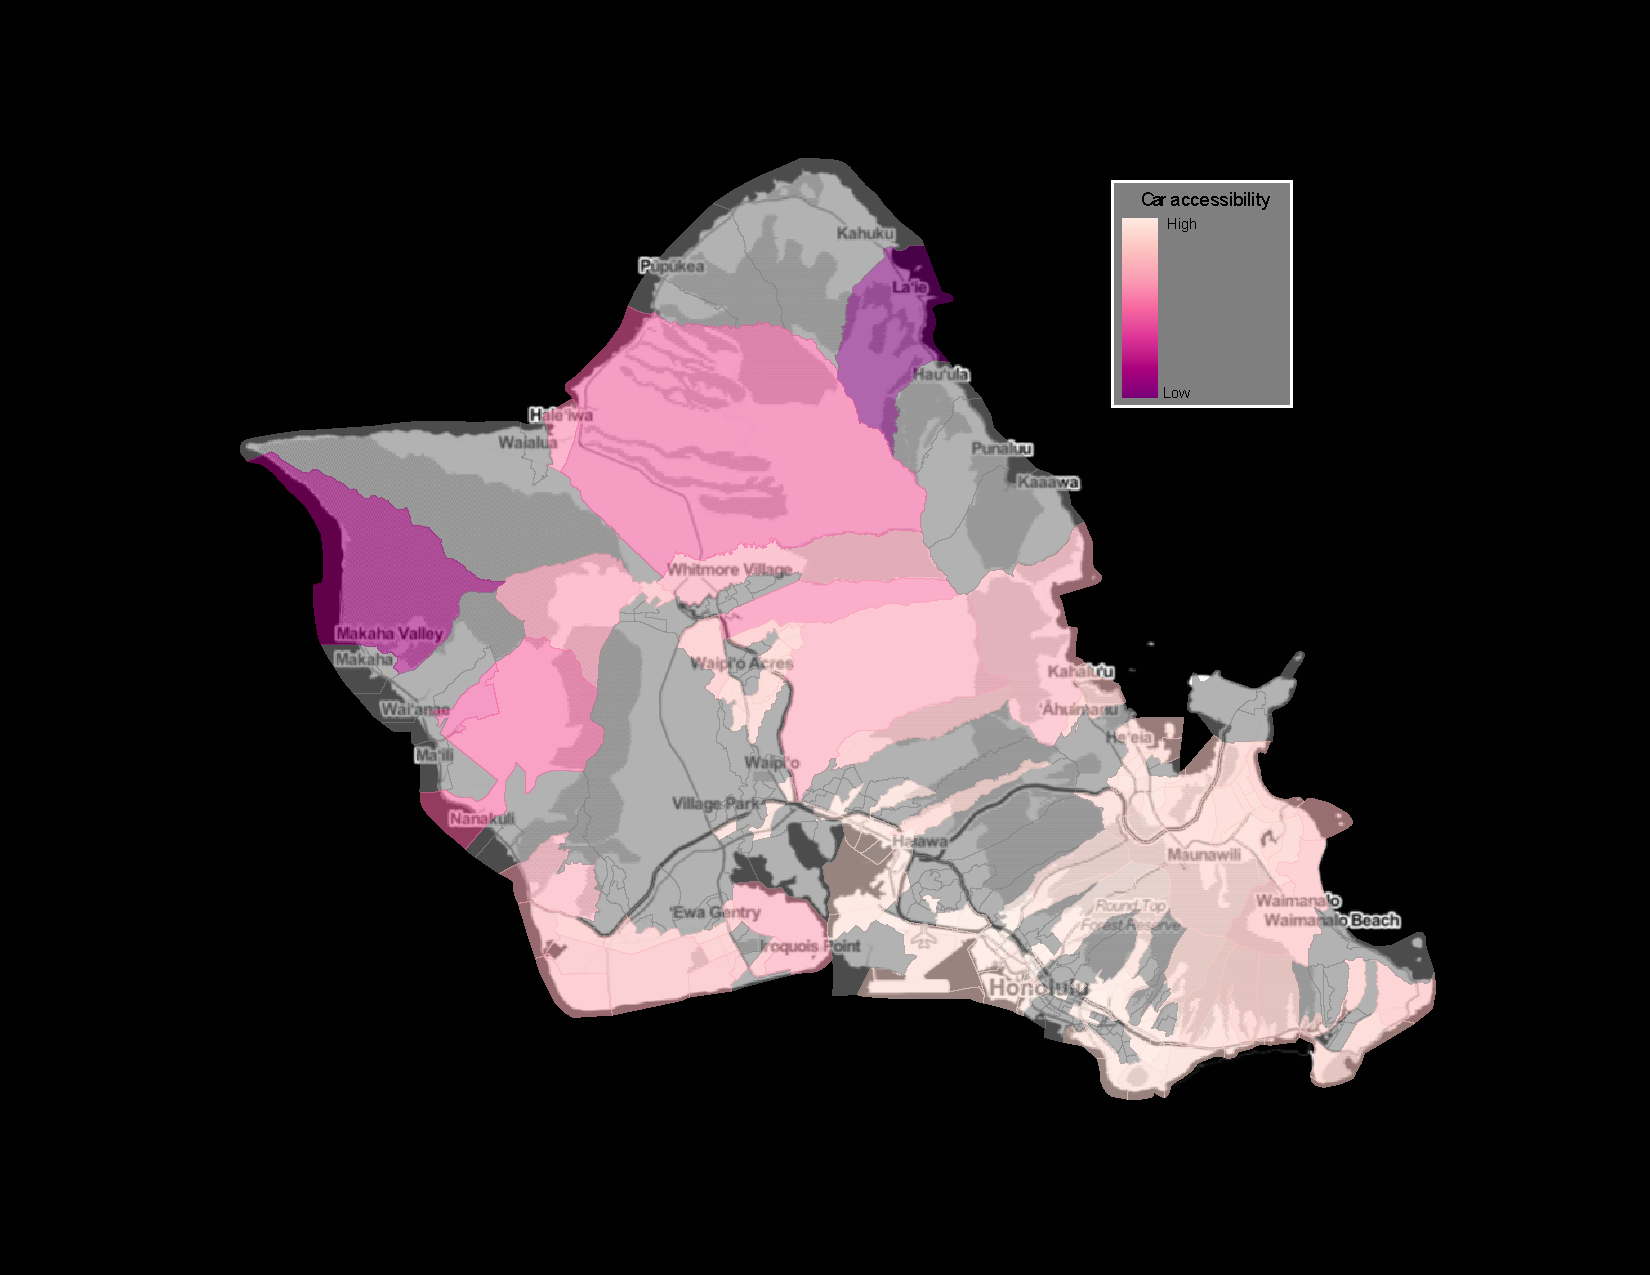
\includegraphics[width=1\linewidth]{car_access} 

}

\caption{Spatialization of car accessibility.}\label{fig:figurename6}
\end{figure}

\begin{figure}

{\centering 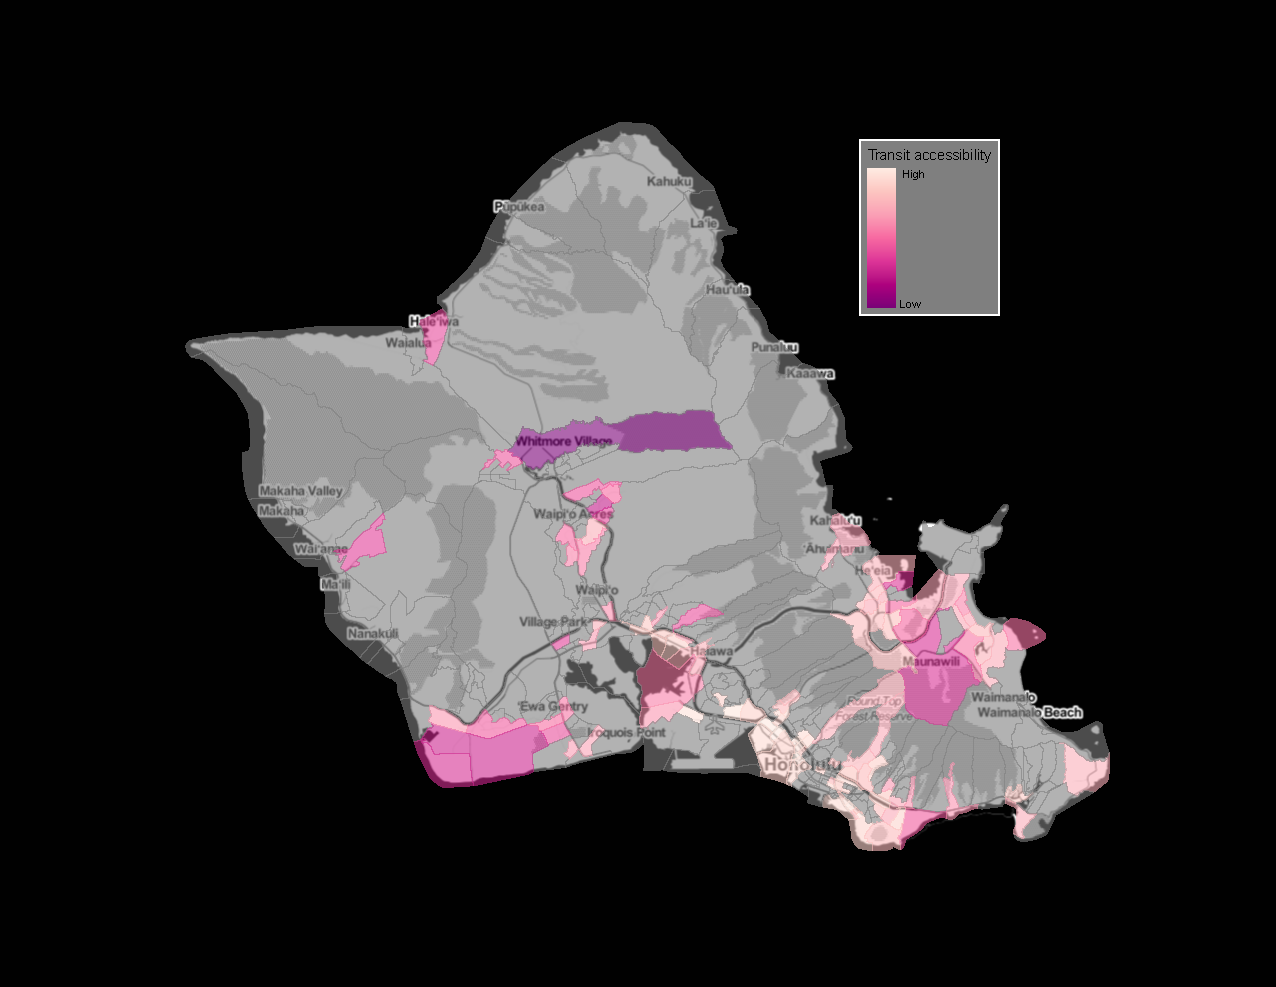
\includegraphics[width=1\linewidth]{transit_access} 

}

\caption{Spatialization of transit accessibility.}\label{fig:figurename7}
\end{figure}

The results of this exercise showed some interesting trends when
factoring employment as the accessibility factor rather than just
showing what travel is possible from one census tract to another.

Generally, we would expect to see a high level of access centered around
downtown, with the accessibility decreasing as distance from downtown
increases. However, there are tracts directly adjacent to downtown that
don't even register on the accessibility index; while at the same time,
there are tracts on the other side of the island that have high levels
of accessibility. So, instead of a continuous scale of decreasing
accessibility as distance increases from downtown, we see a patchwork
map that almost indicates a binary variable for accessibility: the
destinations are either accessible to some degree, or not at all. Even
in the access by car map, we see a very random distribution of levels in
access.

This can tell us a lot about where employment centers are concentrated
throughout the island. Unsurprisingly, the transit accessibility map
further filters down these employment centers. Although they are still
scattered throughout the island, many more tracts are left empty.
indicating that people commuting to those areas for work do not have the
option of public transit.

\end{document}
